\documentclass{letter}
\usepackage[colorlinks=true, urlcolor=blue]{hyperref}
\usepackage{amsbsy}
\usepackage{amssymb}
\usepackage{graphicx}
\usepackage{color}
\usepackage{physics}
\usepackage{soul}
\usepackage{color}
\usepackage{bm}
\usepackage[normalem]{ulem}
\usepackage{verbatim}
\usepackage{natbib}
\usepackage{graphicx}
\pagestyle{empty}
\longindentation=0pt

\begin{document}
\begin{letter}{}
\vspace*{-11\baselineskip}
\opening{}




{\bf Summary of changes in response to referees' comments:}
\begin{enumerate}
\item Update the SI with the full proof for the derivation of the entropy production of the system. 
\item Include error analysis in the all the simulations' measurements. 
\item  Emphasize on the physical sense of the equations as well as its applicability.

\end{enumerate}

{\bf Referee 1 comments:}
\newline
{
My main criticism is about the relevance of the model. The authors do 
not provide any justification for the employed model. In fact, they 
justify the model by referring to previous studies of 2D membranes. 
The authors make here a clear overstatement. They do not present a 2D 
model of a membrane but rather a ring model. Compare for example with 
the 2D model in ref 29 (used by the authors in page 2 as a 
justification for the model), which is a true 2D model. I agree -of 
course- that 2D models are relevant in the study of the physics of 
membranes, as clearly demonstrated by the literature in the field. But 
the model presented here is a toy model which is simply a ring with a 
variable number of particles interacting with a spring with their two 
nearest neighbors. This is not a model of a 2D membrane.

 The relevance of the model presented here has to be clearly justified. 
As it is, the present work describes a very simple toy model of an 
elastic system that allows a detailed study of nonequilibrium 
thermodynamics, a question of interest for specialized physicists 
working in nonequilibrium systems. But the actual relevance of the 
model and the findings for the more general audience of PRL remain to 
be clearly described.
}

\textit{ \bf We thank the referee for bring up this point. At the beginning of this study, we were looking for a minimal model to help us applying the principles of stochastmic thermodynamics to the problem of membrane growth. We choose this model because of several reasons. The first reason is that despite its simplicity of the model, it has been used as benchmark for many studies in membranes. We were actually motivated by the paper of Leibler, Singh, and Fisher$^1$ who first used this model to gain more insights into membrane behaviors. Their paper then inspired many following papers$^{2,3,4,5}$  which use similar models to study membranes with both analytical results and simulations. The second reason is that even though the equilibrium of this model is well studied, not many has investigated the effect of non-equilibrium forces such as growing the system from an extra chemical potential like we do. Traditionally, to describe this non-equilibrium effect one will have to write down detailed hydrodynamic equations such as mass transfer, and momentum transfer. In this paper, we have illustrated that with the development of stochastic thermodynamics, one can write down instead thermodynamics like equations to capture these non-equilibrium phenomena. Thus, with this well-known model, we hope to highlight the advantages of using stochastic themodynamics to diverse groups of audiences. In addition, the 3D membrane model also follows many characteristics of the simpler 2D one. We have illustrated these results of the 3D membrane model as part of our reply to the third referee below ({\bf \it cite Figure number}). Finally, in the proof that we have added to the SI, even though we have used chemical potentials as the non-equilibrium drive, this does not have to be the only case. One can substitute the extra chemical potential to other non-equilibrium driving force extending our results other cases such as proteins induced membrane’s shape. We, thus, believe that the results in our paper is suitable for the more general audience of PRL.} 


{\bf Referee 2 comments:}

  The authors study a very simple problem, just a single ring polymer 
with only local interactions. It is a highly idealized system to work 
with, something like a toy problem. From this point of view, both the 
simulation method and the results obtained seem trivial. 

{\bf We thank the referee for bringing this point up. {\it Maybe we can avoid saying it is not trivial etc and just focus of what we are contributing ? }Despite the apparent simplicity of the model, we don't think it is an trivial task to write down analytical hydrodynamic equations such as mass transfer, momentum transfer to describe the phenomenon here which is the traditional approach in studying these non-equilibrium effect. The highlight of our paper is that instead of using this approach, one can adopt the results of stochastic thermodynamics to write out thermodynamics like equation even for non-equilibrium system with relative ease. }

What is by far more interesting is the theoretical analysis. 
However, the authors use several assumptions and refer quite often to 
previous papers or treatments. For example, how For example, how one 
goes from Eq. (7) to Eq. (8) is not explained. With respect to Eq. 
(8), an interesting point to discuss is if such a nonequilibrium 
system, there exists a well defined diffusion constant D with respect 
to the size fluctuations of the assembly system.

{\bf We thank the referee for bringing this point up.  We have added a detailed proof for the derivation of Eq. 7 in the SI. Eq. 8 is an extension to the Thermodynamics Uncertainty Relation. Thus we can then extend the proof for the Thermodyanmics Uncertainty Relation to our proof in the SI to obtain Eq. 8.} 

Also unclear is how Eq. (10) is obtained. There are several 
assumptions involved such as (e.g.) that the bending rigidity remains 
close to its equilibrium value. 

{\bf We thank the referee for bringing this up. We have also emphasized how Eq. 10 is obtained in the SI. Briefly, from the simulations we know that the system here is well described using the form of Helfrich Hamiltonian for both the equilibrium case and non-equilibrium case but with a normalized surface tension term{\it what about bending?}. From simulation results shown in Fig. 3 of the main text, the bending rigidity does not seem to change much with increasing chemical potential. With these, one can use the {\it why can you say this ?}$E_{\rm eq} = \sum \left ( \gamma_{\rm eq} q^2+\kappa_{\rm eq} q^4\right)|h(q)|^2$ and $E_{\rm eff} = \sum \left ( \gamma_{\rm eff} q^2+\kappa_{\rm eq} q^4\right)|h(q)|^2$ together with their respective $F_{\rm eq}$ and $F_{\rm eff}$ and plug in Eq. 7 in the main text to arrive at Eq. 10 } 

As a result of all these approximations, the authors report that “a 
combination of finite size effects and large fluctuations close to the 
instability lead to the bound for the effective surface tension 
becoming unreliable closer to the instability”. It appears that linear 
response theory and simulations agree well as far as the bound in 
$\delta\mu$ is concerned only close to equilibrium.

{\bf We thank the referee for this comment. We would like to clarify even thought linear response is only valid near equilibrium, our bounds work even at the point of instability as well. {\it provide proof ... talk about how the line in Fig XX shows that the bound works well..Say that this is precisely the point of our result ...usually all people can say/do is linear response, we can go far beyond it...clarify that bound is never violated in our simulations .. even in 3D !!..clarify that bound requires minimal kinetic information...no matter what protocol you use to add and remove, our thing should work !!! } Unfortunately, because of the increased fluctuation near the instability, it is very tough to pin point the exact point of the instability through our simulations. The bounds, however, do relatively well in indicating the point of instability as shown in our Fig. 6.  } 

{\bf Referee 3 comments:}

 What kind of quantity is $<\epsilon_{diss}>$ ? Despite its central 
importance in the manuscript, there is no discussion of how to think 
about this quantity. Since it is the mediating quantity between $\delta 
\mu$ and the effective material constants $\gamma_{eff}$ and 
$\kappa_{eff}$, it seems important to give an intuitive and physical 
idea about what it is. 

{\bf We thank the referee for bringing this up. We have updated the text to emphasize on the role of $<\epsilon_{diss}>$. Briefly, when the components in a bath, in this case the particles, are in saturation with its assembly counter part, the equilibrium chemical potential as well as the structures the assembly adopts at equilibrium is dictated by the energy landscape $E_{\rm eq}$. $<\epsilon_{diss}>$ then can be considered as the minimum work required to change equilibrium energy landscape to $E_{\rm eq}$ to a new one $E_{\rm eff}$. In our paper, the driving force for this change is the extra chemical potential $\delta\mu$ we put in the bath but this does not have to be the only case.}

Similarly, “Eq. 7 and Eq. 8 can be used to predict bounds on how 
$\gamma_{eff}$ changes with the nonequilibrium driving $\delta \mu$” 
(presumably using Equation 10). But what exactly is that bound? 
$<\epsilon_{diss}>$ depends in a quite complicated way on $\gamma_{eff}$, so without further discussion and explicit equation(s), it’s not 
obvious how to understand the bound. 

{\bf We thank the referee for bringing this up. We have updated the text to disscuss more about the physical properties of Eq. 7 and 8. In short, Eq. 7 is the second law of thermodynamics for this process. This resulted have been obtained by using the principles of stochastic thermodynamics as detailted in the proof in our SI. Eq. 8 is the Thermodynamics Uncertainty Relation which has been written for the self-assembly process.}

It is not sufficient to simply state that the results are not affected 
by choices of $N_0$ and $t_{measure}$ (p.3 top left); this should be 
explicitly and systematically shown. Likewise, the reader can’t just 
take the authors’ word that $\gamma_{eff}$, $\kappa_{eff}$, $\mu_{coex}$, 
and $\delta \mu_c$ are time- and size-independent; this should be shown

{\bf We thank the referee for pointing this out. We have updated the manuscript to indicate that Fig. 2 shows the fluctuations of assembly at different $N_0$ which are all overlap to each other. For reference, we also attach Fig. 2 below }

\begin{minipage}{\textwidth}
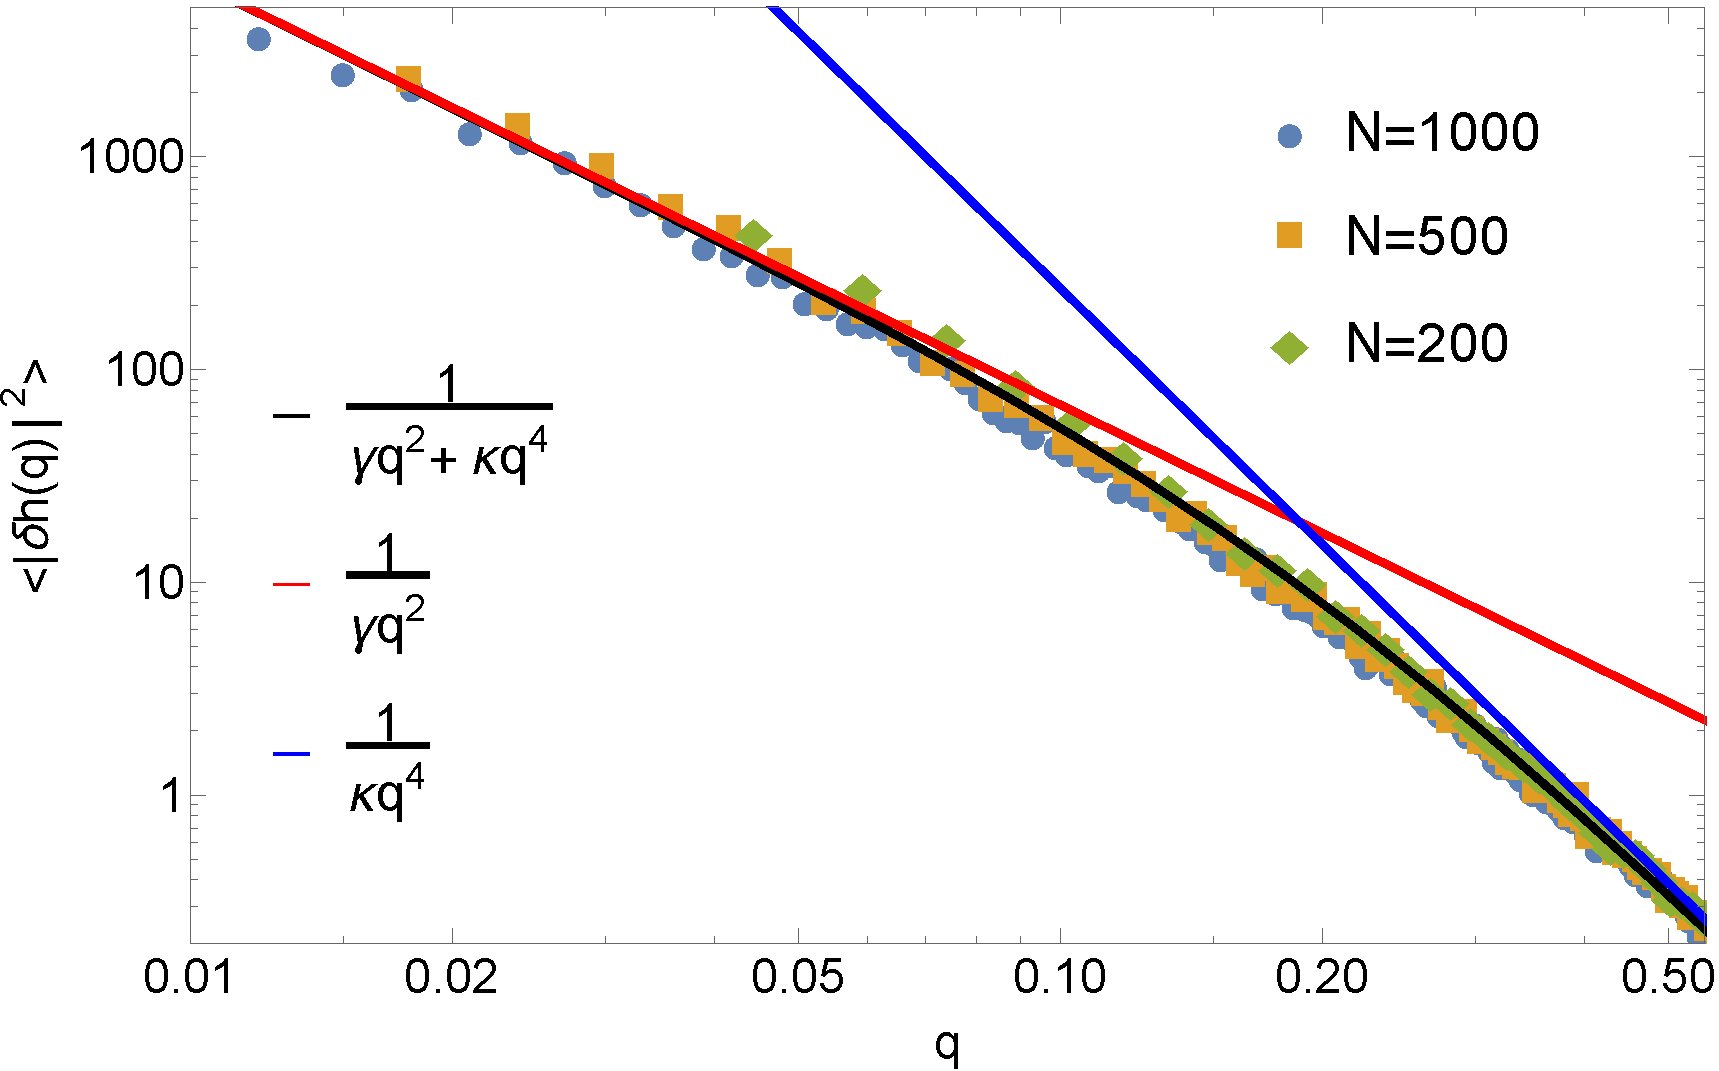
\includegraphics[scale=0.35]{scalingindependentofsizeFig2.pdf}
\centering
\end{minipage}
{\bf This figure shows the power spectrum of interfacial fluctuations at equilibrium. For small wavevectors, q, $|\delta h(q)|^2\propto q^{-2}$ while $|\delta h(q)|^2\propto q^{-4}$ at high q in agreement. The data here is for $k_s=4$ and $k_\theta = 6$. The diamond symbols are fluctuations of the assembly with 200 particles. The square symbols are fluctuations of the assembly with 500 particles. The circle symbols are fluctuation of the assembly with 1000 particles. Because the fluctuations here follow the Helfrich Hamiltonian, its standard deviation is exactly equal to its average magnitude due to the exponential nature of the distribution.}


There is no error analysis in any of the data plots. 

{\bf We thank the referee for pointing this out. We have included error analysis in all the plots.}

Multiple figures are missing crucial details that would ease their 
interpretation. I make several suggestions in “More information 
needed”, below. 

{\bf
We thank the referee for the suggestion. We have updated the figures accordingly. }

I would like more detail on the proposed generalizability of these 
findings to three dimensions. In particular, on p.2, top left, the 
authors write that “this elastic model possesses many features $[26–29, 31–34]$ characteristic of three-dimensional membranes”. Please 
explicitly summarize some of these features. I think it is important 
to at least speculate on what features are expected to generalize (and 
the rationale for this), and which are specific features of the 
two-dimensional geometry. 

{\bf
We thank the referee for the suggestion. We have added some preliminary results for the 3D membrane in the SI. We also list the results below:
{\it provide referene for 3D model ...say we will include this data in upcoming work}Similarly to the 2D model, we triangulate the particles in the 3D and let them interact according to the Hamiltonian $H=\sum (k_A(A-A_0)^2 + k_\theta (\theta-\pi/3)^2 + k_\phi (\phi-\pi)^2$), here A is the area that three particles make, $\theta$ is the angle they make and $\phi$ is the angle that two adjacent planes make}

\begin{minipage}{\textwidth}
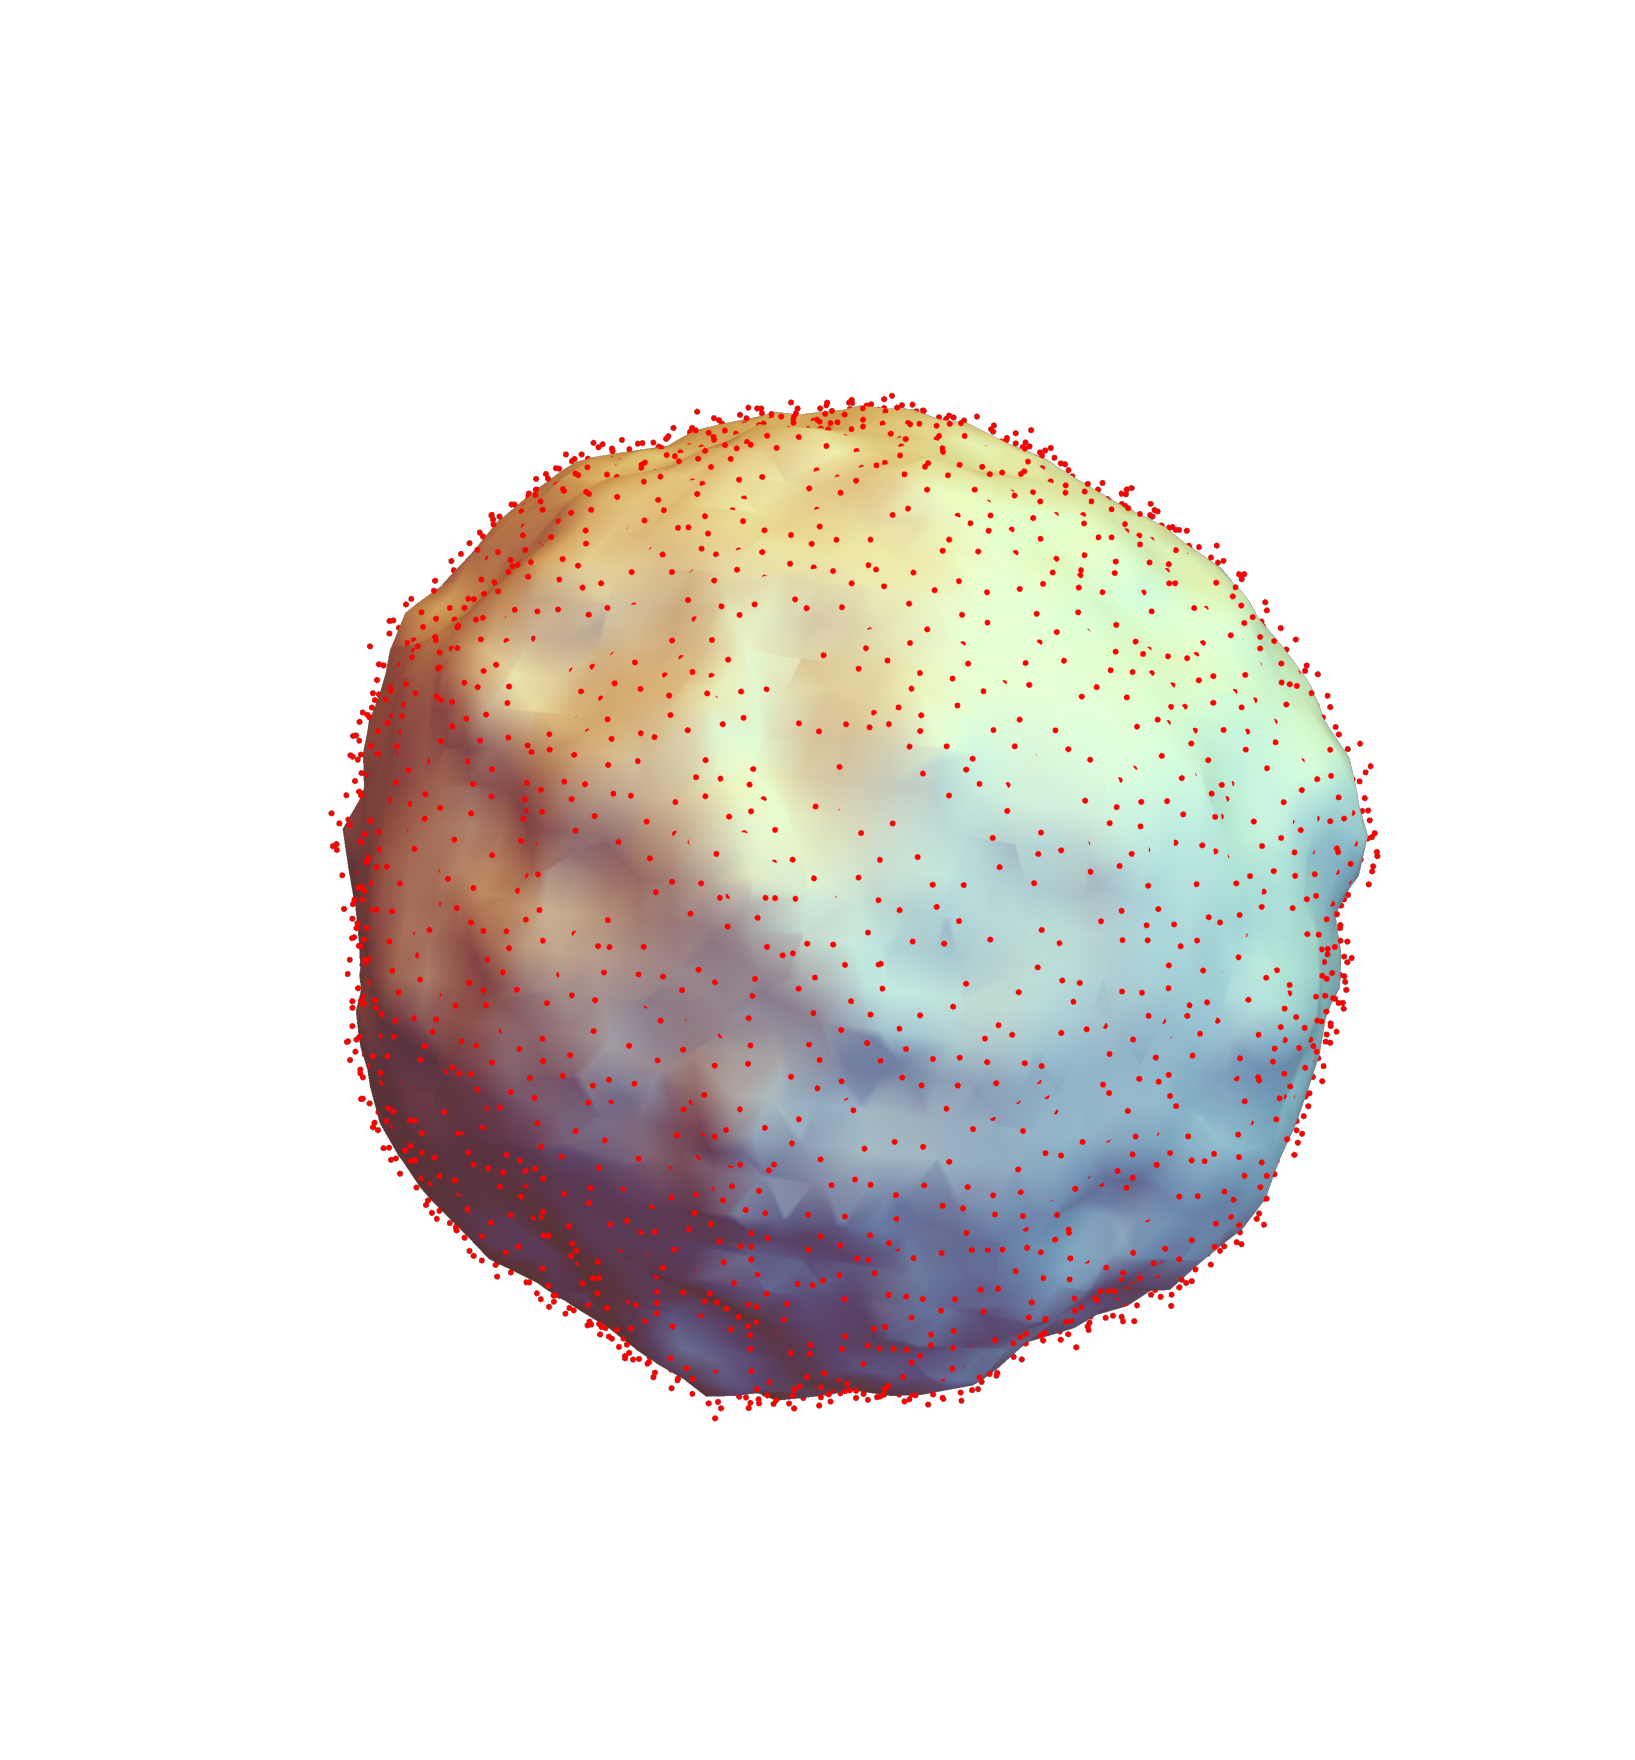
\includegraphics[scale=0.35]{3DMembraneShapeProjectedSurface.pdf}
\centering
\end{minipage}

{\bf
This figure shows the shape of our 3D Membrane model}

\begin{minipage}{\textwidth}
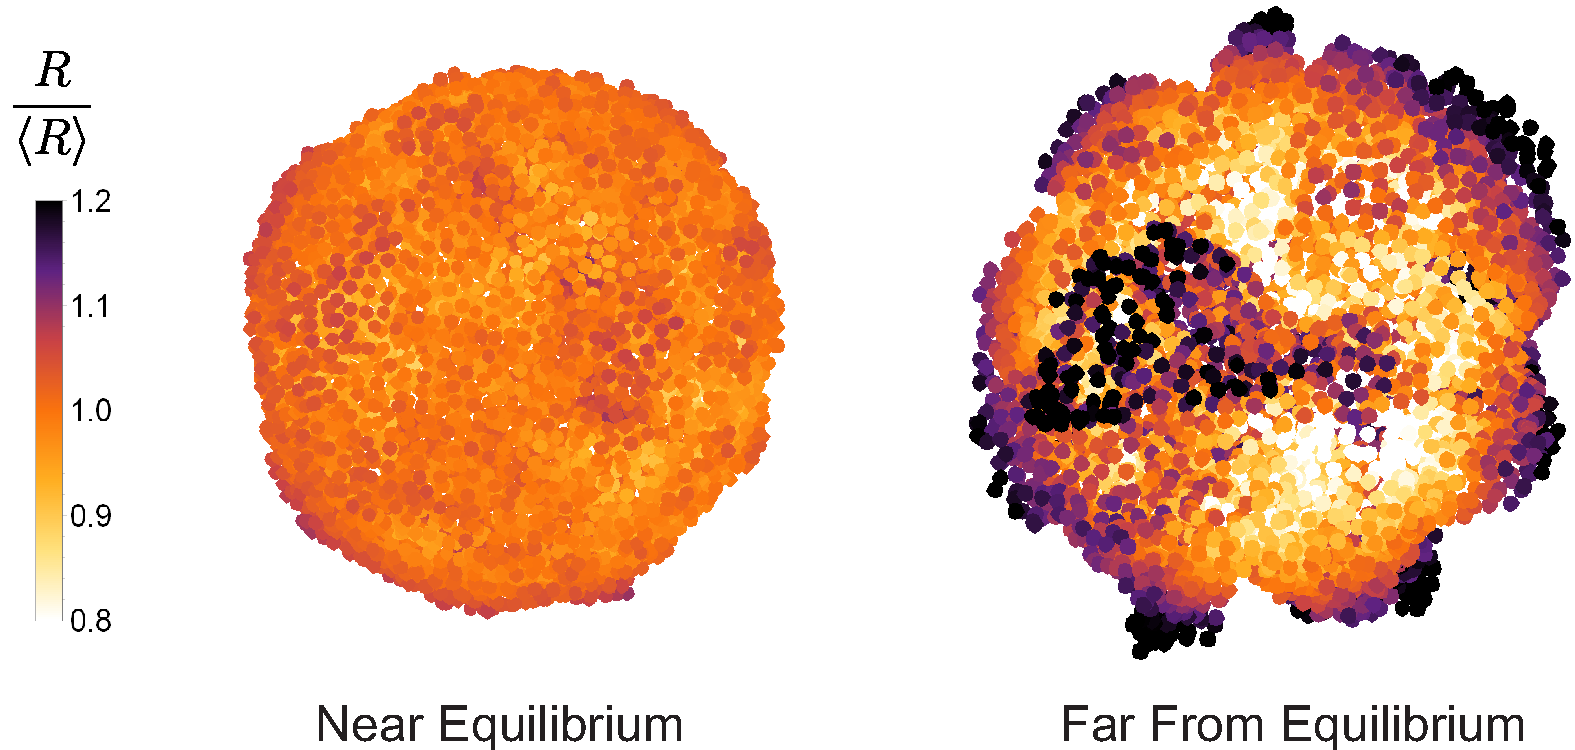
\includegraphics[scale=0.35]{3DMembraneRelativeRadius.pdf}
\centering
\end{minipage}

{\bf
This figure shows the heat map for the relative position of each particle to the average radius of the membrane. In figure in the membrane at near equilibrium while the one in the right is far from equilibrium. We see that similar instability is observed here.}

\begin{minipage}{\textwidth}
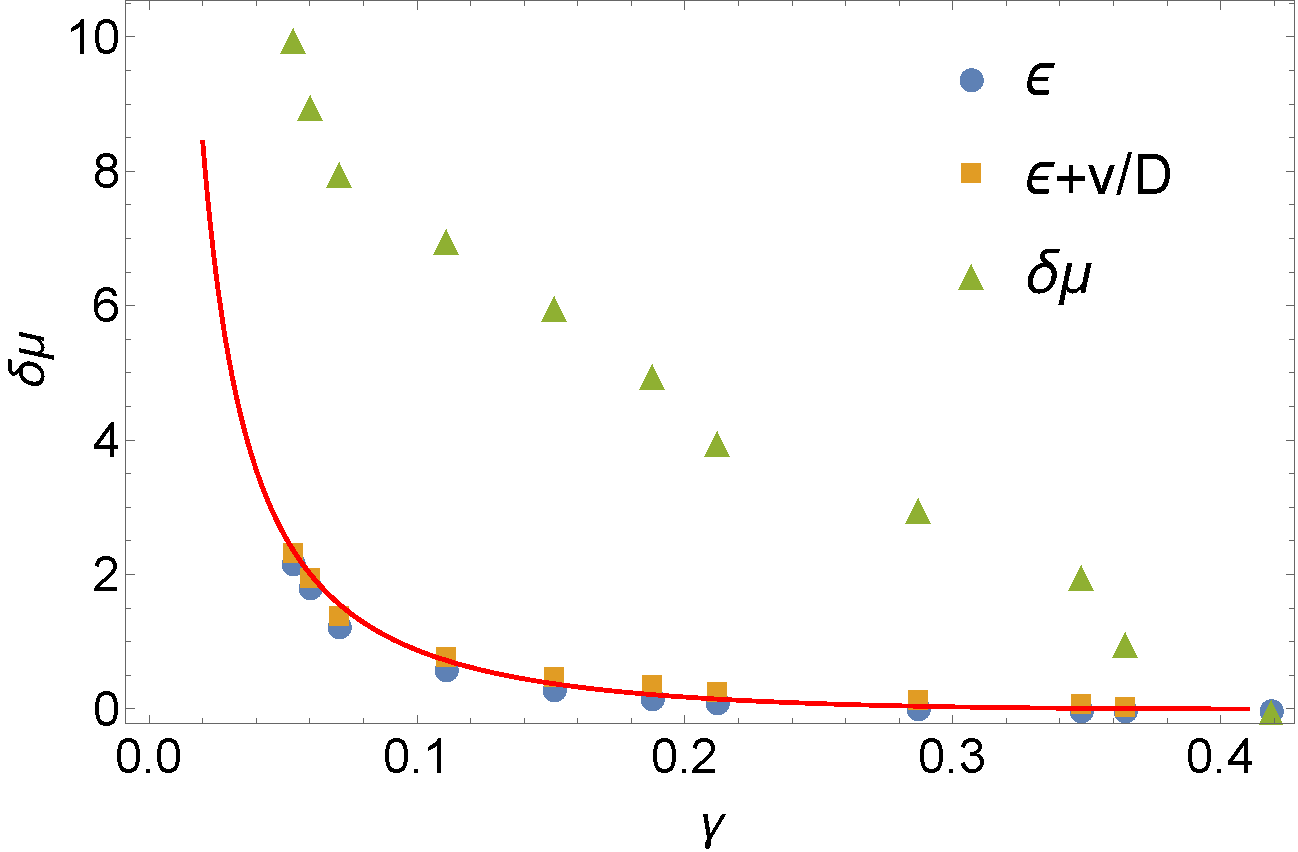
\includegraphics[scale=0.35]{boundsfor3Dmembrane.pdf}
\centering
\end{minipage}
{\bf
This figure is similar to Fig. 6 in the main text but for 3D model. In here, however, it seems the contribution of v/D is minimal. We are still investigating why this happen. }

Clarification 
p.3, top left: $n\langle l\rangle$ is a distance, but $x_n$ seems to be treated as an 
angle. Please resolve the apparent inconsistency here. Regardless, 
$n<l>$ does not give the position (angle) of the nth particle, but 
rather the nth evenly spaced position (angle). 

{\bf
We thank the referee for noticing this. In order to simplifying the discrete Fourier Transform technique, we have assumed that the all the particles are evenly spaced by the distance $<l> $which is the average distance between the particles. This assumption should be valid as long as the assembly remains circular.}

p.3, bottom left: At equilibrium, what is the expected relation 
between your input parameters $k_s$ and $k_{\theta}$ and the Helfrich 
parameters $\gamma$ and $\kappa$?

{\bf
At equilibrium, the $k_s$ is inversely proportional to $\gamma$ and does not affect $\kappa$. $k_\theta$ has a nonlinear relation with $\gamma$ and $\kappa$. Simulations indicate that as $k_\theta$ goes up, $\gamma$ increase while $\kappa$ decrease. }

p.4 bottom left: “In the limit of slow growth where the effective 
elastic constants are minimally renormalized, δμ ≫ εdiss”. In this 
limit, both $\delta\mu$ and $\epsilon_{diss}$ are small. What is the 
general argument about why $\delta \mu >> \epsilon_{diss}$ ? 

{\bf

In the limit of $\delta\mu$ is small, the result of linear response dominates $\delta\mu \approx v/D$. Since $\delta\mu -\epsilon_{diss} \geq v/D$. This makes $\epsilon_{diss}$ very small comparing the $\delta\mu$. In Fig 6, we have plotted $\epsilon_{diss}$ and compare to actual $\delta\mu$ in the simulation. }


p.4 bottom right: why do you say that the bound is unreliable? It 
looks like it is looser, but it doesn’t appear to be violated. 

{\bf
We thank the referee for pointing this out. We have clarified this in our newest manuscript. The reason we say this is because it not easy to pin point the exact point of instability in simulation. Thus, we are unsure how close our prediction to the actual simulation. The bound, however, should still work.} 

SI p.1 bottom left: If “the way we increment time” is any but the most 
ordinary method (constant amount per step), it is not explicitly 
discussed in the text. From what I can gather, you seem to be 
incrementing time in a completely vanilla fashion, but it is the 
timescale for accepting attempted particle insertions that leads to N 
growing as $\sqrt{t}$. If so, this should be made clearer in the text. 

{\bf
We thank the referee for pointing this out. We have updated our manuscript to clarify this. But briefly, in this simulation the number of particles are growing unlike the normal Monte Carlo simulation. In the normal Monte Carlo simulations, where the average number of particles in the system is constant, it is simple to relate time in the vanilla fashion, each Monte Carlo move, to the time as in each Monte Carlo sweep. In this system, where the number of particle is increasing, this relation is no longer simple related. As the referee said, it is the accepting attempted particle insertions that leads to N growing as $\sqrt{t}$ where t here is the incrementing time in each Monte Carlo move. But if we were to switch the time to each Monte Carlo Sweep, then N will now grow as t not as $\sqrt{t}$}

The simulation methodology doesn’t appear to obey the appropriate 
(generalized) detailed balance condition. How do you choose where to 
put E? I.e., for a given B and C, there are many places to add E, 
whereas for a given B, C, and E, there is only one move that removes 
E. Thus it’s not obvious why the proposal probabilities don’t appear 
in your acceptance criteria, if your moves are to obey generalized 
detailed balance. 

{\bf
{\it maybe you can also point to our proof which shows that entropy production is proportional to  growth rate. Hence we can identify delta mu=0 as a point where growth rate is zero and entropy production is zero. The answer below doesn't seem to address the question about acceptance criteria ... Can you say something about that ? }We thank the referee for pointing this out. Instead of considering B and C, we consider all B, C and E as a condition. For the points, B and C, there are indeed many places to give E. We then consider that in the assembly, if we sample many times, there will be a lot of configurations B,C and E' ( here E' doesn't have to be exactly E) that with the removal of E' resulted in B and C. In addition, the moves in these simulations are only addition and removal, thus when the assembly doesn't grow, these are the only moves that can cancel out exactly.}

SI Eq. 3: why should the effects you list enter in the form that you 
write down here? 

SI Fig 2: what are the fit parameter values? 

SI Fig 3: * Legend is missing label. * If you independently fit the 
two clouds, what do you get? 

{\bf
We thank the referee for pointing this out. We have updated the SI to further clarify this. Briefly, We use the form in Eq. 3 as a fit for our growth. The square root form is due to the way we increment time in our simulations and the accepting time scale of particle insertion. The other constants are there because of initial conditions: the initial number of particles and the starting time. We have updated the figure and include in the fit parameters as the referee suggested. We have also listed the fitted results for the two clouds in the main text.}

SI p.2 top right: “we can construct an effective fluctuation of the 
interface when it is out of equilibrium”. I don’t know what this 
means. 

It’s not clear what is the distinction between SI Fig. 4 and main-text 
Fig. 6. 
{\bf
We thank the referee for pointing this out. In the main text, we have used the bounds to ask the question: given a new $\gamma_{\rm eff}$ what is the minimum $\delta\mu$ for this to be true, and that is what Fig. 6 in the main text show. In the SI, we ask the question, given a $\delta\mu$, what is the least deviate $\lambda_{\rm eff}$ that the system will adopt when it is out of equilibrium, and this is what SI. Fig 4 shows.}

More information needed: 

Manuscript is inconsistent about including kT or setting to 1, often 
without explicitly informing the reader. 
Every SI section should be referenced in a relevant location in the 
main text. As it stands, there is crucial information in the SI that 
one would not be aware of on just reading the main text. 
SI must distinguish explicitly between SI Figures and main-text 
Figures. 

{\bf
We thank the referee for these commends. We have updated the manuscript and the SI as the referee’s suggestions.}

Please give more guidance about where Equations 4, 5, 8, and 10 come 
from, otherwise the reader can’t independently judge them.

{\bf
We thank the referee for these suggestions, we have added a proof and further explained on these equations}

\section{References}
\begin{enumerate}
\item S. Leibler, R. R. P. Singh, and M. E. Fisher, Phys. Rev. Lett. 59, 1989 (1987). \item M. E. Fisher, Physica D: Nonlinear Phenomena 38, 112 (1989).
\item J. Rudnick and G. Gaspari, Science (1991). 
\item M. K. Mitra, G. I. Menon, and R. Rajesh, Phys. Rev. E 77, 041802 (2008). 
\item E. Katifori, S. Alben, and D. R. Nelson, Phys. Rev. E 79, 056604 (2009).
\end{enumerate}
Regards,
Michael Nguyen\\
Suriyanarayanan Vaikuntanathan (Corresponding Author)   \\
Email: \href{mailto:svaikunt@uchicago.edu}{svaikunt@uchicago.edu}

\end{letter}
\end{document}
